\section{Kernels}\label{kernels}

The operating system kernel is a special piece of software. This is the
piece of software that is loaded up before all of your other programs
even consider getting booted up. What the kernel does is the following,
abbreviated

\begin{enumerate}
\def\labelenumi{\arabic{enumi}.}
\tightlist
\item
  The operating system executes ROM or read only code
\item
  The operating system then executes a \texttt{boot\_loader} or
  \texttt{EFI} extensions nowadays
\item
  The boot\_loader loads your kernels
\item
  Your kernel executes \texttt{init} to
  \href{https://en.wikipedia.org/wiki/Bootstrapping}{bootstrap} itself
  from nothing
\item
  The kernel executes start up scripts
\item
  The kernel executes userland scripts, and you get to use your
  computer!
\end{enumerate}

You don't need to know the specifics of the booting process, but there
it is. When you are executing in user space the kernel provides some
important operations that programs don't have to worry about. *
Scheduling Processes and threads; in addition, handling synchronization
primitives * Providing System Calls like \texttt{write} or \texttt{read}
* Manages virtual memory and low level binary devices like \texttt{usb}
drivers * Handles reading and understanding a filesystem * Handles
communicating over networks * Handles communications with other
processes * Dynamically linking libraries

The kernel handles all of this stuff in kernel mode. Kernel mode gets
you greater power, like executing extra CPU instructions but at the cost
of one failure crashes your entire computer -- ouch. That is what you
are going to interacting with in this class.

\subsubsection{File Descriptors}\label{file-descriptors}

One of the things that you have already become familiar with is that the
kernel gives you file descriptors when you open text files. Here is a
zine from Julia Evans that details it a bit.

\begin{figure}[htbp]
\centering
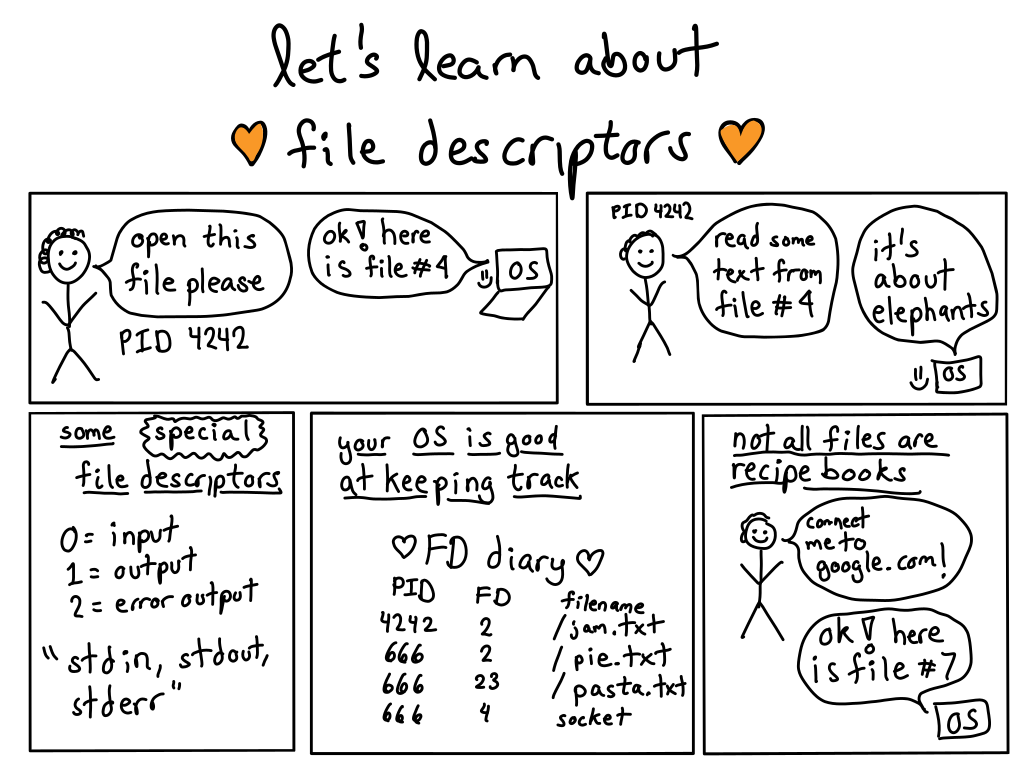
\includegraphics{https://drawings.jvns.ca/drawings/file-descriptors.svg}
\caption{Fds}
\end{figure}

As the little zine shows, the Kernel keeps track of the file descriptors
and what they point to. We will see later that file descriptors need not
point to actual files and the OS keeps track of them for you. Also,
notice that between processes file descriptors may be reused but inside
of a process they are unique.

File descriptors also have a notion of position. You can read a file on
disk completely because the OS keeps track of the position in the file,
and that belongs to your process as well.

\subsection{Cool, what's a shell then?}\label{cool-whats-a-shell-then}

A shell is actually how you are going to be interacting with the kernel.
Before User Friendly operating systems, when a computer started up all
you had access to was a shell. This meant that all of your commands and
editing had to be done this way. Nowadays, our computers start up in
desktop mode, but one can still access a shell using a terminal. When
you open one up you should see something like this

\begin{verbatim}
(Stuff) $
\end{verbatim}

It is ready for your next command! You can type in a lot of unix
utilities like \texttt{ls}, \texttt{echo\ Hello} and the shell will
execute them and give you the result. Some of these are what are known
as \texttt{shell-builtins} meaning that the code is in the shell program
itself. Some of these are compiled programs that you run. The shell only
looks through a special variable called path which contains a list of
\texttt{:} separated paths to search for an executable with your name,
here is an example path.

\begin{verbatim}
$ echo $PATH
/usr/local/sbin:/usr/local/bin:/usr/sbin:/usr/bin:/sbin:/bin:/usr/games:/usr/local/games
\end{verbatim}

So when the shell executes \texttt{ls}, it looks through all of those
directories, finds \texttt{/bin/ls} and executes that.

\begin{verbatim}
$ ls
...
$ /bin/ls
\end{verbatim}

You can always call through the full path. That is always why in past
classes if you want to run something on the terminal you've had to do
\texttt{./exe} because typically the directory that you are working in
is not in the \texttt{PATH} variable. The \texttt{.} expands to your
current directory and your shell executes
\texttt{\textless{}current\_dir\textgreater{}/exe} which is a valid
command.

\subsubsection{Shell tricks and tips}\label{shell-tricks-and-tips}

\begin{itemize}
\tightlist
\item
  The up arrow will get you your most recent command
\item
  \texttt{ctrl-r} will search commands that you previously ran
\item
  \texttt{ctrl-c} will interrupt your shell's process
\item
  Add more!
\end{itemize}

\subsection{Alright then what's a
terminal?}\label{alright-then-whats-a-terminal}

A terminal is just an application that displays the output form the
shell. You can have your default terminal, a quake based terminal,
terminator, the options are endless!

\subsection{Processes}\label{processes}

A process is program that is running, kinda. A process is also just one
instance of that computer program running. Processes have a lot of
things at their disposal. At the start of each program you get one
process, but each program can make more processes. In fact, your
operating system starts up with only one process and all other processes
are forked off of that -- all of that is done under the hood when
booting up.

\subsection{Okay, but what's a program?}\label{okay-but-whats-a-program}

Programs usually contain the following * A binary format: This tells the
operating system which set of bits in the binary are what -- which part
is executable, which parts are constants, which libraries to include
etc. * A set of machine instructions * A number denoting which
instruction to start from * Constants * Libraries to link and where to
fill in the address of those libraries

\subsection{In the beginning}\label{in-the-beginning}

When your operating system starts on a linux machine, there is a process
called \texttt{init.d} that gets created. That process is a special one
handling signals, interrupts, and a persistence module for certain
kernel elements. Whenever you want to make a new process, you call
\texttt{fork} (to be discussed in a later section) and use another
function to load another program.

\subsection{Process Isolation}\label{process-isolation}

Processes are very powerful but they are isolated! That means that by
default, no process can communicate with another process. This is very
important because if you have a large system (let's say EWS) then you
want some processes to have higher privileges (monitoring, admin) than
your average user, and one certainly doesn't want the average user to be
able to bring down the entire system either on purpose or accidentally
by modifying a process.

If I run the following code,

\begin{verbatim}
int secrets; //maybe defined in the kernel or else where
secrets++;
printf("%d\n", secrets);
\end{verbatim}

On two different terminals, as you would guess they would both print out
1 not 2. Even if we changed the code to do something really hacky (apart
from reading the memory directly) there would be no way to change
another process' state (okay maybe
\href{https://en.wikipedia.org/wiki/Dirty_COW}{this} but that is getting
a little too in depth).

\section{Process Contents}\label{process-contents}

\subsection{Memory Layout}\label{memory-layout}

When a process starts, it gets its own address space. Meaning that each
process gets : * \textbf{A Stack}. The Stack is the place where
automatic variable and function call return addresses are stored. Every
time a new variable is declared, the program moves the stack pointer
down to reserve space for the variable. This segment of the stack is
Writable but not executable. If the stack grows too far -- meaning that
it either grows beyond a preset boundary or intersects the heap -- you
will get a stackoverflow most likely resulting in a SEGFAULT or
something similar. \textbf{The stack is statically allocated by default
meaning that there is only a certain amount of space to which one can
write} * \textbf{A Heap}. The heap is an expanding region of memory. If
you want to allocate a large object, it goes here. The heap starts at
the top of the text segment and grows upward (meaning sometimes when you
call \texttt{malloc} that it asks the operating system to push the heap
boundary upward). This area is also Writable but not Executable. One can
run out of heap memory if the system is constrained or if you run out of
addresses (more common on a 32bit system). * \textbf{A Data Segment}
This contains all of your globals. This section starts at the end of the
text segment and is static in size because the amount of globals is
known at compile time. There are two areas to the data usually the
\textbf{IBSS} and the \textbf{UBSS} which stand for the initialized
basic service set and the uninitialized data segment respectively. This
section is Writable but not Executable and there isn't anything else too
fancy here. * \textbf{A Text Segment}. This is, arguably, the most
important section of the address. This is where all your code is stored.
Since assembly compiles to 1's and 0's, this is where the 1's and 0's
get stored. The program counter moves through this segment executing
instructions and moving down the next instruction. It is important to
note that this is the only Executable section of the code. If you try to
change the code while it's running, most likely you will segfault (there
are ways around it but just assume that it segfaults). * Why doesn't it
start at zero? It is outside the
\href{https://en.wikipedia.org/wiki/Address_space_layout_randomization}{scope}
of this class but it is for security.

\subsection{Process ID (PID)}\label{process-id-pid}

To keep track of all these processes, your operating system gives each
process a number and that process is called the PID, process ID.
Processes also have a \texttt{ppid} which is short for parent process
id. Every process has a parent, that parent could be \texttt{init.d}

Processes could also contain * Running State - Whether a process is
getting ready, running, stopped, terminated etc. * File Descriptors -
List of mappings from integers to real devices (files, usb sticks,
sockets) * Permissions - What \texttt{user} the file is running on and
what \texttt{group} the process belongs to. The process can then only do
this admissible to the \texttt{user} or \texttt{group} like opening a
file that the \texttt{user} has made exclusives. There are tricks to
make a program not be the user who started the program i.e.
\texttt{sudo} takes a program that a \texttt{user} starts and executes
it as \texttt{root}. * Arguments - a list of strings that tell your
program what parameters to run under * Environment List - a list of
strings in the form \texttt{NAME=VALUE} that one can modify.

\subsection{A word of warning}\label{a-word-of-warning}

Process forking is a very powerful (and very dangerous) tool. If you
mess up and cause a fork bomb (explained later on this page),
\textbf{you can bring down the entire system}. To reduce the chances of
this, limit your maximum number of processes to a small number e.g 40 by
typing \texttt{ulimit\ -u\ 40} into a command line. Note that this limit
is only for the user, which means if you fork bomb, then you won't be
able to kill all of the processes you just created since calling
\texttt{killall} requires your shell to fork() \ldots{} ironic right? So
what can we do about this. One solution is to spawn another shell
instance as another user (for example root) before hand and kill
processes from there. Another is to use the built in \texttt{exec}
command to kill all the user processes (careful you only have one shot
at this). Finally you could reboot the system :)

When testing fork() code, ensure that you have either root and/or
physical access to the machine involved. If you must work on fork ()
code remotely, remember that \textbf{kill -9 -1} will save you in the
event of an emergency.

TL;DR: Fork can be \textbf{extremely} dangerous if you aren't prepared
for it. \textbf{You have been warned.}

\section{Intro to Fork}\label{intro-to-fork}

\subsection{What does fork do?}\label{what-does-fork-do}

The \texttt{fork} system call clones the current process to create a new
process. It creates a new process (the child process) by duplicating the
state of the existing process with a few minor differences (discussed
below). The child process does not start from main. Instead it returns
from \texttt{fork()} just as the parent process does.

Just as a side remark, in older UNIX systems, the entire address space
of the parent process was directly copied (regardless of whether the
resource was modified or not). These days, kernel performs
\href{https://en.wikipedia.org/wiki/Copy-on-write}{copy-on-write}, which
saves a lot of resources, while being very time efficient. \#\# What is
the simplest \texttt{fork()} example? Here's a very simple
example\ldots{}

\begin{verbatim}
printf("I'm printed once!\n");
fork();
// Now there are two processes running
// and each process will print out the next line.
printf("You see this line twice!\n");
\end{verbatim}

\subsection{Why does this example print 42
twice?}\label{why-does-this-example-print-42-twice}

The following program prints out 42 twice - but the \texttt{fork()} is
after the \texttt{printf}!? Why?

\begin{verbatim}
#include <unistd.h> /*fork declared here*/
#include <stdio.h> /* printf declared here*/
int main() {
   int answer = 84 >> 1;
   printf("Answer: %d", answer);
   fork();
   return 0;
}
\end{verbatim}

The \texttt{printf} line \emph{is} executed only once however notice
that the printed contents is not flushed to standard out (there's no
newline printed, we didn't call \texttt{fflush}, or change the buffering
mode). The output text is therefore still in process memory waiting to
be sent. When \texttt{fork()} is executed the entire process memory is
duplicated including the buffer. Thus the child process starts with a
non-empty output buffer which will be flushed when the program exits.

\subsection{How do you write code that is different for the parent and
child
process?}\label{how-do-you-write-code-that-is-different-for-the-parent-and-child-process}

Check the return value of \texttt{fork()}.

If fork() returns -1, that implies something went wrong in the process
of creating a new child. One should check the value stored in
\emph{errno} to determine what kind of error occurred; commons one
include EAGAIN and ENOMEM (check
\href{http://www-numi.fnal.gov/offline_software/srt_public_context/WebDocs/Errors/unix_system_errors.html}{this
page} to get a description of the errors).

Similarly, a return value of 0 indicates that we are in the child
process, while a positive integer shows that we are in parent process.
The positive value returned by fork() gives as the process id
(\emph{pid}) of the child.

Here's one way to remember which is which:

The child process can find its parent - the original process that was
duplicated - by calling \texttt{getppid()} - so does not need any
additional return information from \texttt{fork()}. The parent process
however can only find out the id of the new child process from the
return value of \texttt{fork}:

\begin{verbatim}
pid_t id = fork();
if (id == -1) exit(1); // fork failed 
if (id > 0)
{ 
// I'm the original parent and 
// I just created a child process with id 'id'
// Use waitpid to wait for the child to finish
} else { // returned zero
// I must be the newly made child process
}
\end{verbatim}

\subsection{What is a fork bomb ?}\label{what-is-a-fork-bomb}

A `fork bomb' is when you attempt to create an infinite number of
processes. A simple example is shown below:

\begin{verbatim}
while (1) fork();
\end{verbatim}

This will often bring a system to a near-standstill as it attempts to
allocate CPU time and memory to a very large number of processes that
are ready to run. Comment: System administrators don't like fork-bombs
and may set upper limits on the number of processes each user can have
or may revoke login rights because it creates a disturbance in the force
for other users' programs. You can also limit the number of child
processes created by using \texttt{setrlimit()}.

fork bombs are not necessarily malicious - they occasionally occur due
to student coding errors.

Angrave suggests that the Matrix trilogy, where the machine and man
finally work together to defeat the multiplying Agent-Smith, was a
cinematic plot based on an AI-driven fork-bomb.

\section{Waiting and Execing}\label{waiting-and-execing}

\subsection{How does the parent process wait for the child to
finish?}\label{how-does-the-parent-process-wait-for-the-child-to-finish}

Use \texttt{waitpid} (or \texttt{wait}).

\begin{verbatim}
pid_t child_id = fork();
if (child_id == -1) { perror("fork"); exit(EXIT_FAILURE);}
if (child_id > 0) { 
  // We have a child! Get their exit code
  int status; 
  waitpid( child_id, &status, 0 );
  // code not shown to get exit status from child
} else { // In child ...
  // start calculation
  exit(123);
}
\end{verbatim}

\subsection{Can I make the child process execute another
program?}\label{can-i-make-the-child-process-execute-another-program}

Yes. Use one of the
\href{http://man7.org/linux/man-pages/man3/exec.3.html}{\texttt{exec}}
functions after forking. The \texttt{exec} set of functions replaces the
process image with the the process image of what is being called. This
means that any lines of code after the \texttt{exec} call are replaced.
Any other work you want the child process to do should be done before
the \texttt{exec} call.

The
\href{https://en.wikipedia.org/wiki/Exec_(system_call)\#C_language_prototypes}{Wikipedia
article} does a great job helping you make sense of the names of the
exec family.

The naming schemes can be shortened like this

\begin{quote}
The base of each is exec (execute), followed by one or more letters:

e -- An array of pointers to environment variables is explicitly passed
to the new process image.

l -- Command-line arguments are passed individually (a list) to the
function.

p -- Uses the PATH environment variable to find the file named in the
file argument to be executed.

v -- Command-line arguments are passed to the function as an array
(vector) of pointers.
\end{quote}

\begin{verbatim}
#include <unistd.h>
#include <sys/types.h> 
#include <sys/wait.h>
#include <stdlib.h>
#include <stdio.h>

int main(int argc, char**argv) {
  pid_t child = fork();
  if (child == -1) return EXIT_FAILURE;
  if (child) { /* I have a child! */
    int status;
    waitpid(child , &status ,0);
    return EXIT_SUCCESS;

  } else { /* I am the child */
    // Other versions of exec pass in arguments as arrays
    // Remember first arg is the program name
    // Last arg must be a char pointer to NULL

    execl("/bin/ls", "ls","-alh", (char *) NULL);

    // If we get to this line, something went wrong!
    perror("exec failed!");
  }
}
\end{verbatim}

\subsection{A simpler way to execute another
program}\label{a-simpler-way-to-execute-another-program}

Use \texttt{system}. Here is how to use it:

\begin{verbatim}

#include <unistd.h>
#include <stdlib.h>

int main(int argc, char**argv) {
  system("ls");
  return 0;
}
\end{verbatim}

The \texttt{system} call will fork, execute the command passed by
parameter and the original parent process will wait for this to finish.
This also means that \texttt{system} is a blocking call: The parent
process can't continue until the process started by \texttt{system}
exits. This may or may not be useful. Also, \texttt{system} actually
creates a shell which is then given the string, which is more overhead
than just using \texttt{exec} directly. The standard shell will use the
\texttt{PATH} environment variable to search for a filename that matches
the command. Using system will usually be sufficient for many simple
run-this-command problems but can quickly become limiting for more
complex or subtle problems, and it hides the mechanics of the
fork-exec-wait pattern so we encourage you to learn and use
\texttt{fork} \texttt{exec} and \texttt{waitpid} instead.

\subsection{What is the silliest fork
example?}\label{what-is-the-silliest-fork-example}

A slightly silly example is shown below. What will it print? Try it with
multiple arguments to your program.

\begin{verbatim}
#include <unistd.h>
#include <stdio.h>
int main(int argc, char **argv) {
  pid_t id;
  int status; 
  while (--argc && (id=fork())) {
    waitpid(id,&status,0); /* Wait for child*/
  }
  printf("%d:%s\n", argc, argv[argc]);
  return 0;
}
\end{verbatim}

The amazing parallel apparent-O(N) \emph{sleepsort} is today's silly
winner. First published on
\href{https://dis.4chan.org/read/prog/1295544154}{4chan in 2011}. A
version of this awful but amusing sorting algorithm is shown below.

\begin{verbatim}
int main(int c, char **v)
{
        while (--c > 1 && !fork());
        int val  = atoi(v[c]);
        sleep(val);
        printf("%d\n", val);
        return 0;
}
\end{verbatim}

Note: The algorithm isn't actually O(N) because of how the system
scheduler works. Though there are parallel algorithms that run in
O(log(N)) per process, this is sadly not one of them.

\subsection{What is different in the child process than the parent
process?}\label{what-is-different-in-the-child-process-than-the-parent-process}

The key differences include: * The process id returned by
\texttt{getpid()}. The parent process id returned by \texttt{getppid()}.
* The parent is notified via a signal, SIGCHLD, when the child process
finishes but not vice versa. * The child does not inherit pending
signals or timer alarms. For a complete list see the
\href{http://man7.org/linux/man-pages/man2/fork.2.html}{fork man page}

\section{Do child processes share open
filehandles?}\label{do-child-processes-share-open-filehandles}

Yes! In fact both processes use the same underlying kernel file
descriptor. For example if one process rewinds the random access
position back to the beginning of the file, then both processes are
affected.

Both child and parent should \texttt{close} (or \texttt{fclose}) their
file descriptors or file handle respectively.

\subsection{How can I find out more?}\label{how-can-i-find-out-more}

Read the man pages! *
\href{http://man7.org/linux/man-pages/man2/fork.2.html}{fork} *
\href{http://man7.org/linux/man-pages/man3/exec.3.html}{exec} *
\href{http://man7.org/linux/man-pages/man2/wait.2.html}{wait}

\section{The Pattern}\label{the-pattern}

\subsection{\texorpdfstring{What does the following `exec' example
do?}{What does the following exec example do?}}\label{what-does-the-following-exec-example-do}

\begin{verbatim}
#include <unistd.h>
#include <fcntl.h> // O_CREAT, O_APPEND etc. defined here

int main() {
   close(1); // close standard out
   open("log.txt", O_RDWR | O_CREAT | O_APPEND, S_IRUSR | S_IWUSR);
   puts("Captain's log");
   chdir("/usr/include");
   // execl( executable,  arguments for executable including program name and NULL at the end)

   execl("/bin/ls", /* Remaining items sent to ls*/ "/bin/ls", ".", (char *) NULL); // "ls ."
   perror("exec failed");
   return 0; // Not expected
}
\end{verbatim}

There's no error checking in the above code (we assume close,open,chdir
etc works as expected). * open: will use the lowest available file
descriptor (i.e.~1) ; so standard out now goes to the log file. * chdir
: Change the current directory to /usr/include * execl : Replace the
program image with /bin/ls and call its main() method * perror : We
don't expect to get here - if we did then exec failed.

\subsection{Subtle forkbomb bug}\label{subtle-forkbomb-bug}

What's wrong with this code

\begin{verbatim}
#include <unistd.h>
#define HELLO_NUMBER 10

int main(){
    pid_t children[HELLO_NUMBER];
    int i;
    for(i = 0; i < HELLO_NUMBER; i++){
        pid_t child = fork();
        if(child == -1){
            break;
        }
        if(child == 0){ //I am the child
             execlp("ehco", "echo", "hello", NULL);
        }
        else{
            children[i] = child;
        }
    }

    int j;
    for(j = 0; j < i; j++){
        waitpid(children[j], NULL, 0);
    }
    return 0;
}
\end{verbatim}

We misspelled \texttt{ehco}, so we can't \texttt{exec} it. What does
this mean? Instead of creating 10 processes we just created 2\textbf{10
processes, fork bombing our machine. How could we prevent this? Put an
exit right after exec so in case exec fails we won't end up fork bombing
our machine.}

\subsection{What does the child inherit from the
parent?}\label{what-does-the-child-inherit-from-the-parent}

\begin{itemize}
\tightlist
\item
  Open file handles. If the parent later seeks, say, to the back to the
  beginning of the file then this will affect the child too (and vice
  versa).
\item
  Signal handlers
\item
  Current working directory
\item
  Environment variables
\end{itemize}

See the \href{http://linux.die.net/man/2/fork}{fork man page} for more
details.

\subsection{What is different in the child process than the parent
process?}\label{what-is-different-in-the-child-process-than-the-parent-process-1}

The process id is different. In the child calling \texttt{getppid()}
(notice the two 'p's) will give the same result as calling getpid() in
the parent. See the fork man page for more details.

\subsection{How do I wait for my child to
finish?}\label{how-do-i-wait-for-my-child-to-finish}

Use \texttt{waitpid} or \texttt{wait}. The parent process will pause
until \texttt{wait} (or \texttt{waitpid}) returns. Note this explanation
glosses over the restarting discussion.

\subsection{What is the fork-exec-wait
pattern}\label{what-is-the-fork-exec-wait-pattern}

A common programming pattern is to call \texttt{fork} followed by
\texttt{exec} and \texttt{wait}. The original process calls fork, which
creates a child process. The child process then uses exec to start
execution of a new program. Meanwhile the parent uses \texttt{wait} (or
\texttt{waitpid}) to wait for the child process to finish. See below for
a complete code example.

\subsection{How do I start a background process that runs at the same
time?}\label{how-do-i-start-a-background-process-that-runs-at-the-same-time}

Don't wait for them! Your parent process can continue to execute code
without having to wait for the child process. Note in practice
background processes can also be disconnected from the parent's input
and output streams by calling \texttt{close} on the open file
descriptors before calling exec.

However child processes that finish before their parent finishes can
become zombies. See the zombie page for more information.

\section{Zombies}\label{zombies}

\subsection{Good parents don't let their children become
zombies!}\label{good-parents-dont-let-their-children-become-zombies}

Note, the word `zombie' in this instance sheds some light as to what
they actually represent. When a child finishes (or terminates) it still
takes up a slot in the kernel process table. Furthermore, they still
contain information about the process that got terminated, such as
process id, exit status, etc. (i.e.~a skeleton of the original process
still remains). Only when the child has been `waited on' will the slot
be available and the remaining information can be accessed by the
parent.

A long running program could create many zombies by continually creating
processes and never \texttt{wait}-ing for them.

\subsection{What would be effect of too many
zombies?}\label{what-would-be-effect-of-too-many-zombies}

Eventually there would be insufficient space in the kernel process table
to create a new processes. Thus \texttt{fork()} would fail and could
make the system difficult / impossible to use - for example just logging
in requires a new process!

\subsection{What does the system do to help prevent
zombies?}\label{what-does-the-system-do-to-help-prevent-zombies}

Once a process completes, any of its children will be assigned to
``init'' - the first process with pid of 1. Thus these children would
see getppid() return a value of 1. These orphans will eventually finish
and for a brief moment become a zombie. Fortunately, the init process
automatically waits for all of its children, thus removing these zombies
from the system.

\subsection{How do I prevent zombies? (Warning: Simplified
answer)}\label{how-do-i-prevent-zombies-warning-simplified-answer}

Wait on your child!

\begin{verbatim}
waitpid(child, &status, 0); // Clean up and wait for my child process to finish.
\end{verbatim}

Note we assume that the only reason to get a SIGCHLD event is that a
child has finished (this is not quite true - see man page for more
details).

A robust implementation would also check for interrupted status and
include the above in a loop. Read on for a discussion of a more robust
implementation.

\subsection{How can I asynchronously wait for my child using SIGCHLD?
(ADVANCED)}\label{how-can-i-asynchronously-wait-for-my-child-using-sigchld-advanced}

Warning: This section uses signals which we have not yet fully
introduced. The parent gets the signal SIGCHLD when a child completes,
so the signal handler can wait on the process. A slightly simplified
version is shown below.

\begin{verbatim}
pid_t child;

void cleanup(int signal) {
  int status;
  waitpid(child, &status, 0);
  write(1,"cleanup!\n",9);
}
int main() {
   // Register signal handler BEFORE the child can finish
   signal(SIGCHLD, cleanup); // or better - sigaction
   child = fork();
   if (child == -1) { exit(EXIT_FAILURE);}

   if (child == 0) { /* I am the child!*/
     // Do background stuff e.g. call exec   
   } else { /* I'm the parent! */
      sleep(4); // so we can see the cleanup
      puts("Parent is done");
   }
   return 0;
} 
\end{verbatim}

The above example however misses a couple of subtle points: * More than
one child may have finished but the parent will only get one SIGCHLD
signal (signals are not queued) * SIGCHLD signals can be sent for other
reasons (e.g.~a child process is temporarily stopped)

A more robust code to reap zombies is shown below.

\begin{verbatim}
void cleanup(int signal) {
  int status;
  while (waitpid((pid_t) (-1), 0, WNOHANG) > 0) {}
}
\end{verbatim}

\subsection{So what are environment
variables?}\label{so-what-are-environment-variables}

Environment variables are variables that the system keeps for all
processes to use. Your system has these set up right now! In Bash, you
can check some of these

\begin{verbatim}
$ echo $HOME
/home/bhuvy
$ echo $PATH
/usr/local/sbin:/usr/bin:...
\end{verbatim}

How would you get these in C/C++? You can use the \texttt{getenv} and
\texttt{setenv} function

\begin{verbatim}
char* home = getenv("HOME"); // Will return /home/bhuvy
setenv("HOME", "/home/bhuvan", 1 /*set overwrite to true*/ );
\end{verbatim}

\subsection{Right, so how do these environment variables mean anything
to
parent/child?}\label{right-so-how-do-these-environment-variables-mean-anything-to-parentchild}

Well each process gets its own dictionary of environment variables that
are copied over to the child. Meaning, if the parent changes their
environment variables it won't be transferred to the child and vice
versa. This is important in the fork-exec-wait trilogy if you want to
exec a program with different environment variables than your parent (or
any other process).

For example, you can write a C program that loops through all of the
time zones and executes the \texttt{date} command to print out the date
and time in all locals. Environment variables are used for all sorts of
programs so modifying them is important.

\section{Wait Macros}\label{wait-macros}

\subsection{Can I find out the exit value of my
child?}\label{can-i-find-out-the-exit-value-of-my-child}

You can find the lowest 8 bits of the child's exit value (the return
value of \texttt{main()} or value included in \texttt{exit()}): Use the
``Wait macros'' - typically you will use ``WIFEXITED'' and
``WEXITSTATUS'' . See \texttt{wait}/\texttt{waitpid} man page for more
information).

\begin{verbatim}
int status;
pid_t child = fork();
if (child == -1) return 1; //Failed
if (child > 0) { /* I am the parent - wait for the child to finish */
  pid_t pid = waitpid(child, &status, 0);
  if (pid != -1 && WIFEXITED(status)) {
     int low8bits = WEXITSTATUS(status);
     printf("Process %d returned %d" , pid, low8bits);
  }
} else { /* I am the child */
 // do something interesting
  execl("/bin/ls", "/bin/ls", ".", (char *) NULL); // "ls ."
}
\end{verbatim}

A process can only have 256 return values, the rest of the bits are
informational.

\subsection{Bit Shifting}\label{bit-shifting}

Note there is no need to memorize this, this is just a high level
overview of how information is stored inside the status variables

From Android source code:

\begin{verbatim}
/* If WIFEXITED(STATUS), the low-order 8 bits of the status. */

#define __WEXITSTATUS(status) (((status) & 0xff00) >> 8)

/* If WIFSIGNALED(STATUS), the terminating signal. */

#define __WTERMSIG(status) ((status) & 0x7f)

/* If WIFSTOPPED(STATUS), the signal that stopped the child. */

#define __WSTOPSIG(status) __WEXITSTATUS(status)

/* Nonzero if STATUS indicates normal termination. */

#define __WIFEXITED(status) (__WTERMSIG(status) == 0)
\end{verbatim}

The kernel has an internal way of keeping track of signaled, exited, or
stopped. That API is abstracted so that that the kernel developers are
free to change at will.

\subsection{Being careful.}\label{being-careful.}

Remember that the the macros only make sense if the precondition is met.
Meaning that a process' exit status won't be defined if the process is
signaled. The macros will not do the checking for you, so it's up to the
programming to make sure the logic checks out.

\section{Signals}\label{signals}

\subsection{What's a signal?}\label{whats-a-signal}

A signal is a construct provided to us by the kernel. It allows one
process to asynchronously send a signal (think a message) to another
process. If that process wants to accept the signal, it can, and then,
for most signals, can decide what to do with that signal. Here is a
short list (non comprehensive) of signals.

\begin{longtable}[c]{@{}lll@{}}
\toprule
\begin{minipage}[b]{0.12\columnwidth}\raggedright\strut
Name
\strut\end{minipage} &
\begin{minipage}[b]{0.44\columnwidth}\raggedright\strut
Default Action
\strut\end{minipage} &
\begin{minipage}[b]{0.35\columnwidth}\raggedright\strut
Usual Use Case
\strut\end{minipage}\tabularnewline
\midrule
\endhead
\begin{minipage}[t]{0.12\columnwidth}\raggedright\strut
SIGINT
\strut\end{minipage} &
\begin{minipage}[t]{0.44\columnwidth}\raggedright\strut
Terminate Process (Can be caught)
\strut\end{minipage} &
\begin{minipage}[t]{0.35\columnwidth}\raggedright\strut
Tell the process to stop nicely
\strut\end{minipage}\tabularnewline
\begin{minipage}[t]{0.12\columnwidth}\raggedright\strut
SIGQUIT
\strut\end{minipage} &
\begin{minipage}[t]{0.44\columnwidth}\raggedright\strut
Terminate Process (Can be caught)
\strut\end{minipage} &
\begin{minipage}[t]{0.35\columnwidth}\raggedright\strut
Tells the process to stop harshly
\strut\end{minipage}\tabularnewline
\begin{minipage}[t]{0.12\columnwidth}\raggedright\strut
SIGSTOP
\strut\end{minipage} &
\begin{minipage}[t]{0.44\columnwidth}\raggedright\strut
Stop Process (Cannot be caught)
\strut\end{minipage} &
\begin{minipage}[t]{0.35\columnwidth}\raggedright\strut
Stops the process to be continued
\strut\end{minipage}\tabularnewline
\begin{minipage}[t]{0.12\columnwidth}\raggedright\strut
SIGCONT
\strut\end{minipage} &
\begin{minipage}[t]{0.44\columnwidth}\raggedright\strut
Continues a Process
\strut\end{minipage} &
\begin{minipage}[t]{0.35\columnwidth}\raggedright\strut
Continues to run the process
\strut\end{minipage}\tabularnewline
\begin{minipage}[t]{0.12\columnwidth}\raggedright\strut
SIGKILL
\strut\end{minipage} &
\begin{minipage}[t]{0.44\columnwidth}\raggedright\strut
Terminate Process (Cannot be caught)
\strut\end{minipage} &
\begin{minipage}[t]{0.35\columnwidth}\raggedright\strut
You want your process gone
\strut\end{minipage}\tabularnewline
\bottomrule
\end{longtable}

\subsection{When are signals
generated?}\label{when-are-signals-generated}

\begin{itemize}
\tightlist
\item
  When the user sends a signal. For example, you are at the terminal,
  and you send \texttt{CTRL-C}
\item
  When a system event happens. For example, you get a \texttt{SIGCHILD}
  after forking to notice when one of your children have exited.
\item
  When another program sends it. For example, when you execute
  \texttt{kill\ -9\ PID}, it sends \texttt{SIGKILL}
\item
  When an appropriate hardware interrupt is triggered. For example, if
  you access a page that you aren't supposed to, the hardware generates
  a segfault interrupt which gets intercepted by the kernel. The kernel
  finds the process that caused this and sends a software interrupt
  signal \texttt{SIGSEGV}.
\end{itemize}

\subsection{Can I pause my child?}\label{can-i-pause-my-child}

Yes ! You can temporarily pause a running process by sending it a
SIGSTOP signal. If it succeeds it will freeze a process; i.e.~the
process will not be allocated any more CPU time.

To allow a process to resume execution send it the SIGCONT signal.

For example, Here's program that slowly prints a dot every second, up to
59 dots.

\begin{verbatim}
#include <unistd.h>
#include <stdio.h>
int main() {
  printf("My pid is %d\n", getpid() );
  int i = 60;
  while(--i) { 
    write(1, ".",1);
    sleep(1);
  }
  write(1, "Done!",5);
  return 0;
}
\end{verbatim}

We will first start the process in the background (notice the \& at the
end). Then send it a signal from the shell process by using the kill
command.

\begin{verbatim}
>./program &
My pid is 403
...
>kill -SIGSTOP 403
>kill -SIGCONT 403
\end{verbatim}

\subsection{How do I kill/stop/suspend my child from
C?}\label{how-do-i-killstopsuspend-my-child-from-c}

In C, send a signal to the child using \texttt{kill} POSIX call,

\begin{verbatim}
kill(child, SIGUSR1); // Send a user-defined signal
kill(child, SIGSTOP); // Stop the child process (the child cannot prevent this)
kill(child, SIGTERM); // Terminate the child process (the child can prevent this)
kill(child, SIGINT); // Equivalent to CTRL-C (by default closes the process)
\end{verbatim}

As we saw above there is also a kill command available in the shell
e.g.~get a list of running processes and then terminate process 45 and
process 46

\begin{verbatim}
ps
kill -l 
kill -9 45
kill -s TERM 46
\end{verbatim}

\subsection{\texorpdfstring{How can I detect ``CTRL-C'' and clean up
gracefully?}{How can I detect CTRL-C and clean up gracefully?}}\label{how-can-i-detect-ctrl-c-and-clean-up-gracefully}

We will return to signals later on - this is just a short introduction.
On a Linux system, see \texttt{man\ -s7\ signal} if you are interested
in finding out more (for example a list of system and library calls that
are async-signal-safe).

There are strict limitations on the executable code inside a signal
handler. Most library and system calls are not `async-signal-safe' -
they may not be used inside a signal handler because they are not
re-entrant safe. In a single-threaded program, signal handling
momentarily interrupts the program execution to execute the signal
handler code instead. Suppose your original program was interrupted
while executing the library code of \texttt{malloc} ; the memory
structures used by malloc will not be in a consistent state. Calling
\texttt{printf} (which uses \texttt{malloc}) as part of the signal
handler is unsafe and will result in ``undefined behavior'' i.e.~it is
no longer a useful,predictable program. In practice your program might
crash, compute or generate incorrect results or stop functioning
(``deadlock''), depending on exactly what your program was executing
when it was interrupted to execute the signal handler code.

One common use of signal handlers is to set a boolean flag that is
occasionally polled (read) as part of the normal running of the program.
For example,

\begin{verbatim}
int pleaseStop ; // See notes on why "volatile sig_atomic_t" is better

void handle_sigint(int signal) {
  pleaseStop = 1;
}

int main() {
  signal(SIGINT, handle_sigint);
  pleaseStop = 0;
  while ( ! pleaseStop) { 
     /* application logic here */ 
   }
  /* cleanup code here */
}
\end{verbatim}

The above code might appear to be correct on paper. However, we need to
provide a hint to the compiler and to the CPU core that will execute the
\texttt{main()} loop. We need to prevent a compiler optimization: The
expression \texttt{!\ pleaseStop} appears to be a loop invariant
i.e.~true forever, so can be simplified to \texttt{true}. Secondly, we
need to ensure that the value of \texttt{pleaseStop} is not cached using
a CPU register and instead always read from and written to main memory.
The \texttt{sig\_atomic\_t} type implies that all the bits of the
variable can be read or modified as an ``atomic operation'' - a single
uninterruptable operation. It is impossible to read a value that is
composed of some new bit values and old bit values.

By specifying \texttt{pleaseStop} with the correct type
\texttt{volatile\ sig\_atomic\_t} we can write portable code where the
main loop will be exited after the signal handler returns. The
\texttt{sig\_atomic\_t} type can be as large as an \texttt{int} on most
modern platforms but on embedded systems can be as small as a
\texttt{char} and only able to represent (-127 to 127) values.

\begin{verbatim}
volatile sig_atomic_t pleaseStop;
\end{verbatim}

Two examples of this pattern can be found in ``COMP'' a terminal based
1Hz 4bit computer
(https://github.com/gto76/comp-cpp/blob/1bf9a77eaf8f57f7358a316e5bbada97f2dc8987/src/output.c\#L121).
Two boolean flags are used. One to mark the delivery of \texttt{SIGINT}
(CTRL-C), and gracefully shutdown the program, and the other to mark
\texttt{SIGWINCH} signal to detect terminal resize and redraw the entire
display.

\subsection{Topics}\label{topics}

\begin{itemize}
\tightlist
\item
  Correct use of fork, exec and waitpid
\item
  Using exec with a path
\item
  Understanding what fork and exec and waitpid do. E.g. how to use their
  return values.
\item
  SIGKILL vs SIGSTOP vs SIGINT.
\item
  What signal is sent when you press CTRL-C
\item
  Using kill from the shell or the kill POSIX call.
\item
  Process memory isolation.
\item
  Process memory layout (where is the heap, stack etc; invalid memory
  addresses).
\item
  What is a fork bomb, zombie and orphan? How to create/remove them.
\item
  getpid vs getppid
\item
  How to use the WAIT exit status macros WIFEXITED etc.
\end{itemize}

\section{Questions/Exercises}\label{questionsexercises}

\begin{itemize}
\tightlist
\item
  What is the difference between execs with a p and without a p? What
  does the operating system
\item
  How do you pass in command line arguments to \texttt{execl*}? How
  about \texttt{execv*}? What should be the first command line argument
  by convention?
\item
  How do you know if \texttt{exec} or \texttt{fork} failed?
\item
  What is the \texttt{int\ *status} pointer passed into wait? When does
  wait fail?
\item
  What are some differences between \texttt{SIGKILL}, \texttt{SIGSTOP},
  \texttt{SIGCONT}, \texttt{SIGINT}? What are the default behaviors?
  Which ones can you set up a signal handler for?
\item
  What signal is sent when you press \texttt{CTRL-C}?
\item
  My terminal is anchored to PID = 1337 and has just become
  unresponsive. Write me the terminal command and the C code to send
  \texttt{SIGQUIT} to it.
\item
  Can one process alter another processes memory through normal means?
  Why?
\item
  Where is the heap, stack, data, and text segment? Which segments can
  you write to? What are invalid memory addresses?
\item
  Code me up a fork bomb in C (please don't run it).
\item
  What is an orphan? How does it become a zombie? How do I be a good
  parent?
\item
  Don't you hate it when your parents tell you that you can't do
  something? Write me a program that sends \texttt{SIGSTOP} to your
  parent.
\item
  Write a function that fork exec waits an executable, and using the
  wait macros tells me if the process exited normally or if it was
  signaled. If the process exited normally, then print that with the
  return value. If not, then print the signal number that caused the
  process to terminate.
\end{itemize}
